\section{Fibonacci Series}
\subsection{Aim}
To print the fibonacci series and the sum of its odd and even elements

\subsection{Code}
\begin{lstlisting}
DATA SEGMENT
  n DW 8 
  series DW 10 DUP(?)
  sumOdd DW 0
  sumEven DW 0
ENDS DATA   

CODE SEGMENT
ASSUME CS:CODE, DS:DATA
START:
  MOV AX, DATA
  MOV DS, AX
  MOV CX, 00
  MOV BX, 01
  LEA SI, series
  MOV [SI], 00
  ADD SI, 2
  
FIBLOOP:
  MOV AX, CX
  ADD AX, BX
  MOV BX, CX
  MOV CX, AX
  CMP CX, n 
  JG SUMLOOP
  MOV [SI], CX
  ADD SI, 2
  JMP FIBLOOP 
  
SUMLOOP:
  MOV AX, [SI]
  TEST AX, 01H
  JNZ ADDODD
  MOV AX, [SI]
  ADD sumEven, AX
  JMP INCR

ADDODD:
  MOV AX, [SI]
  ADD sumOdd, AX

INCR:
  SUB SI, 2
  CMP SI, series
  JLE EXIT
  JMP SUMLOOP

EXIT:
  MOV AH, 4CH
  INT 21h
ENDS CODE
END START
\end{lstlisting}

\subsection{Output}
\begin{center}
	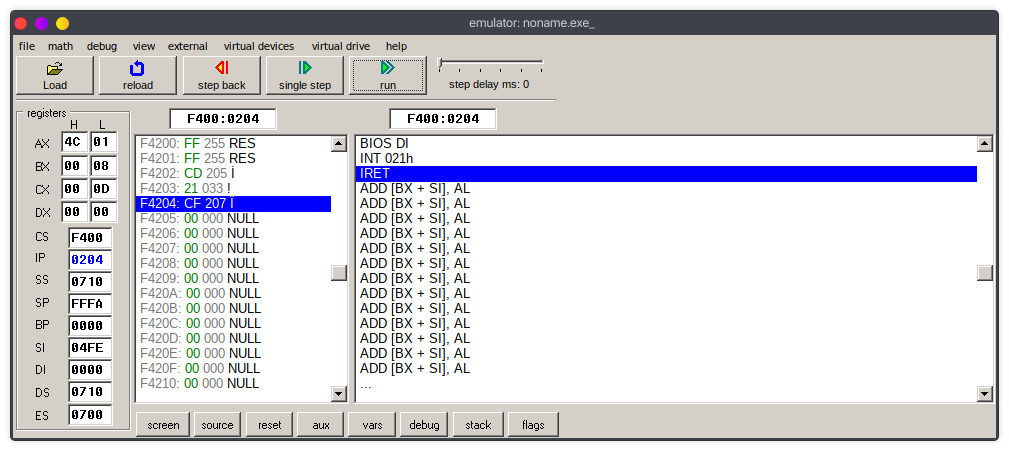
\includegraphics[width=0.90\textwidth]{img/pq1/ss1.png}\\
	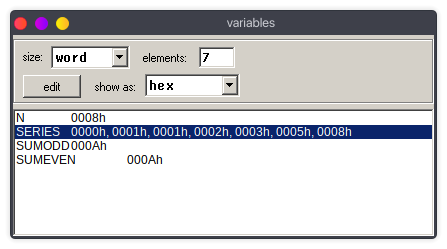
\includegraphics{img/pq1/ss2.png}
\end{center} 

\subsection{Result}
The program for printing fibonacci series was written and its output verified